%% Copyright 2019 Bernd Haberstumpf
%% License: CC BY-NC
% !TeX spellcheck = de_DE
\newsection{Die Geiselnahme}

Haben die Charaktere ihre Nachforschungen in dem St"utzpunkt des Sicherheitsdienstes abgeschlossen sie von Karl Sandos wieder in den Eingangsraum des St"utzpunktes begleitet. Der Spielleiter sollte wenn m"oglich darauf warten das sich die Charaktere au\3erhalb des St"utzpunktes und die im St"utzpunkt in einen Informationsaustausch begeben. Zu diesem Zeitpunkt f"allt die Verbindung "uber das ComNetz pl"otzlich aus. Kurz darauf "offnet sich der Zugang zum St"utzpunkt und ein Gegenstand f"allt in den Raum. Die PAN Netze der Personen im Raum fallen aus. Jeder Charakter in der Station sollte nun einen Konstitutionswurf (Body) machen um nicht kurzzeitig in Ohnmacht zu fallen. Die Funktionen in Systemen des Omegas wenn auf dem St"utzpunkt werden schneller wieder aktiv als bei anderen f"uhren aber zun"achst zu einem Handycap von -4 auf alle physischen W"urfe. Mit dem "offnen des Zugangs zum Eingangsbereich des St"utzpunkt st"urmen zwei bewaffnete Personen in den Raum und beginnen sofort mit vollautomatischen Railguns zu feuern. Befindet sich ein Omega im Eingangsbereich wird er von
Smith Handerson ins Visier genommen. Ein weiteres Ziel ist Karl Sandos der darauf hin hinter dem Tresen zu Boden geht. Ist kein Omega anwesend schie\3t der Angreifer auf einen weiteren Sicherheitsbeamten Luke Lengdon der in die Brust und am Kopf getroffen und ins Koma f"allt. Bei den Angreifern handelt es sich um Slingshot und Smith Handerson. Beide sind in Kampfanz"uge, Smith Handerson mit einem Helm mit Sichtschutz gekleidet. Beim ersten Schu\3wechsel sollte nur ein Omega die M"oglichkeit haben eine Waffe zu ziehen oder in den Nahkampf zu gehen wobei sein Handycap bestehen bleibt. Bei ihrem Angriff sollte es den Angreifern leicht fallen die "uberrumpelten Personen im Eingangsbereich Kampfunf"ahig zu machen und sie danach im Schach halten zu k"onnen. Die Angreifer sammeln die elektronische Schockgranate ein, die die PANs der anwesenden au\3er Kraft gesetzt haben.

W"ahrend die Angreifer den St"utzpunkt "uberfallen um Hanibal zu befreien m"ussen die Charaktere au\3erhalb des St"utzpunktes auf die neue Situation reagieren. Als erstes wollen sie sicher in Erfahrung bringen wo die Verbindung zu ihren Mitstreitern ausgefallen ist. Grace Anders wird in diesem Zusammenhang zuerst versuchen ihren direkten Vorgesetzten Karl Sandos und danach den Sicherheitschef Henk Arongate zu kontaktieren. Von ihm erf"ahrt sie dass nur das ComNetz zum Sicherheitsst"utzpunkt gest"ort ist. Er verspricht Leute zum St"utzpunkt zu schicken weist aber darauf hin das die Ermittler sich am n"ahesten zum St"utzpunkt befinden. Im Umkreis von 50 Metern um den St"utzpunkt herum ist das ComNetz ausgefallen. 

Der St"utzpunkt selbst liegt an einem von zwei Seiten zug"anglichen Tunnel. Vor dem geschlossenen Tor liegt der schwer verletzte Luke Lengdon, nach wie vor nicht ansprechbar. Andere Personen sind nicht erkennbar. Wenn die Charaktere nicht selbst aktiv werden bittet Grace Anders ihr Deckung zu geben und pirscht sich an ihren Ex--Freund heran um dort Ersthilfe zu leisten. Aus dem St"utzpunkt heraus sind keine Ger"ausche zu h"oren. Auf Rufe antwortet niemand. Die T"ur zum St"utzpunkt l"asst sich von au\3en "offnen. Der Eingangsbereich ist auf den ersten Blick hin leer wobei der Tresen nicht einsehbar ist. Auf dem Boden sind blutige Schleifspuren zu erkennen. Um den Tresen herum sind Einschu\3l"ocher zu erkennen. In dieser Situation mu\3 jemand dem verletzten Langdon helfen, den Eingangsbereich des St"utzpunkts und den von beiden angreifbaren Gang absichern. 

\begin{figure*}[htbp]
	\centering
	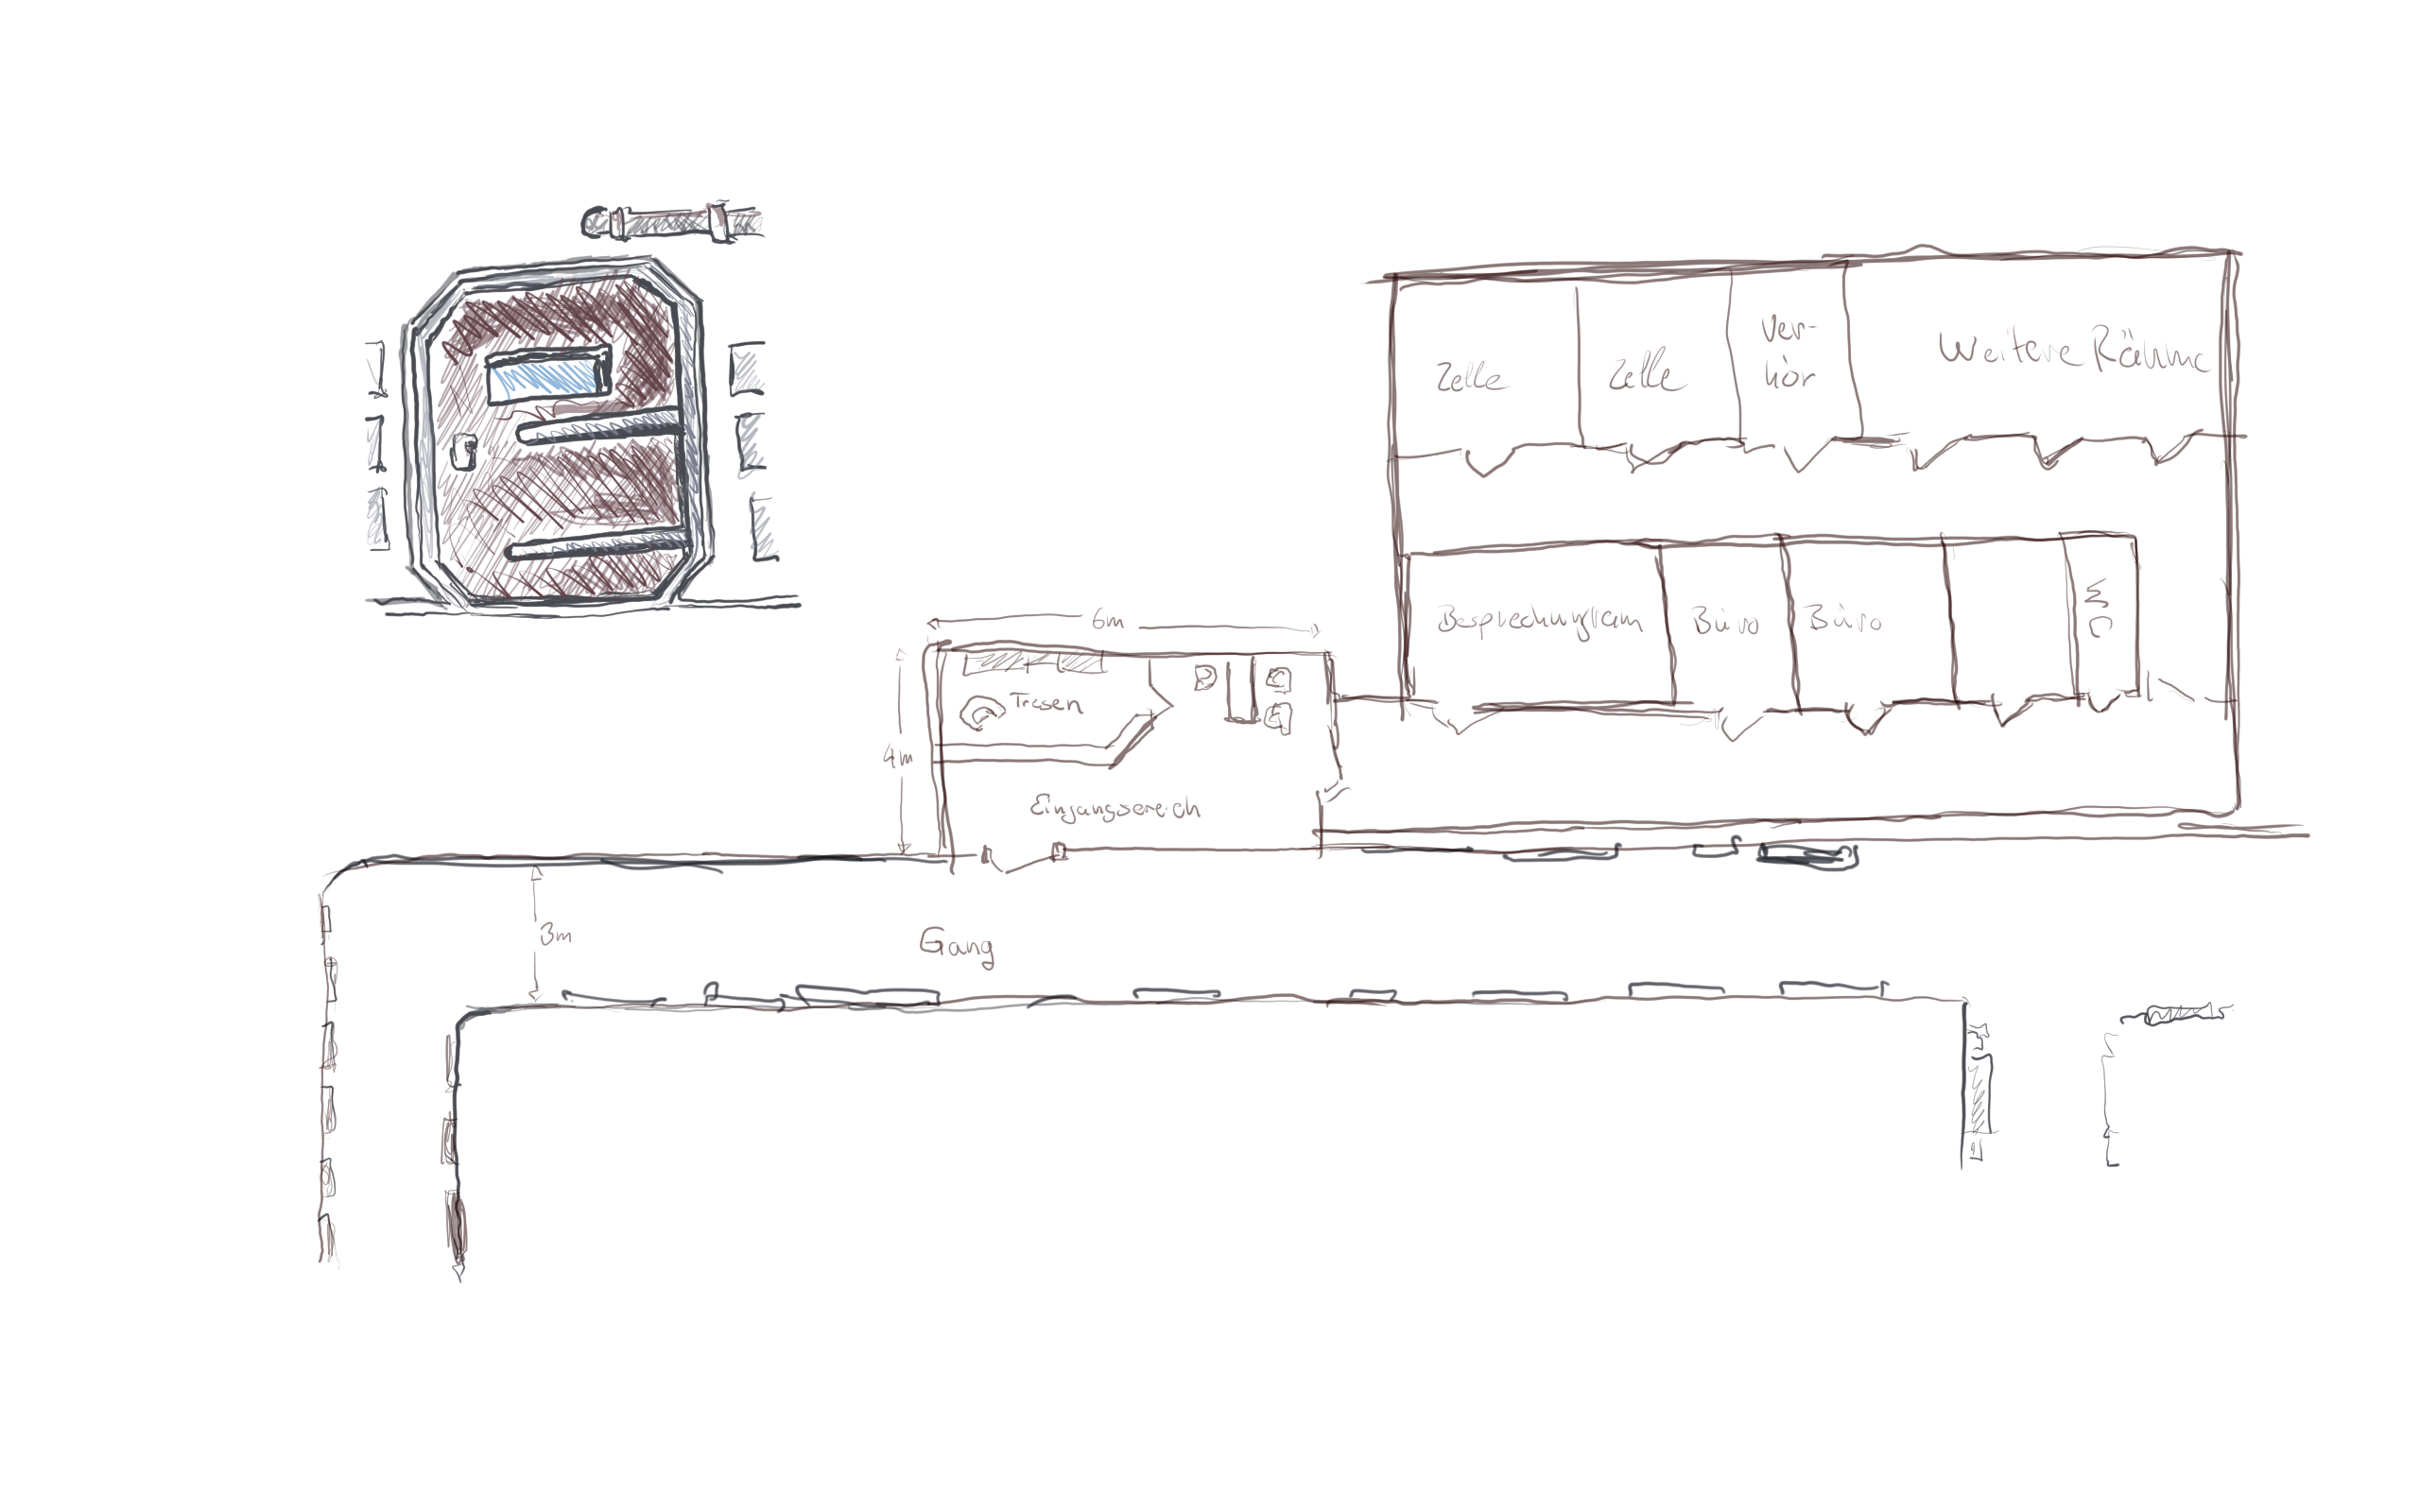
\includegraphics[width=0.9\linewidth]{./images/sicherheitdienst.png}
    \newline{}St"utzpunkt Sicherheitsdienst
	\label{fig:stuetzpunkt-sicherheitsdienst}
\end{figure*}

Zuvor: Wenn Handerson und Slingshot den Eingangsbereich des St"utzpunktes unter Kontrolle haben "offnen sie mit der Chipkarte von Karl Sandos oder Luke Lengdon die T"ur zu den hinteren R"aumlichkeiten, den Gef"angniszellen, dem Verh"orraum und anderen B"uros. Die Angreifer sperren die Charaktere und Karl Sandos in eine Zelle zusammen mit den Minenarbeitern und verlassen den St"utzpunkt mit Hanibal, einem der Charaktere und den beiden Frauen der Minenbesatzung als Geisel. Sie hinterlassen im hinteren Teil des St"utzpunkt einen St"orsender, der das ComNetz in der Umgebung des St"utzpunktes ausschaltet, und ein Funkger"at.  

St"urmen die Ermittler den Eingangsbereich des St"utzpunkts k"onnen sie den Eingangsbereich weiter untersuchen. Der Tresen kann mit einer Chipkarte von Grace Anders betreten werden. Hinter dem Tresen sind weitere Blutspuren zu entdecken. N"ahern sie sich der T"ure in die inneren Bereiche oder versuchen die Attent"ater direkt anzusprechen h"oren sie eine Stimme hinter der T"ure die droht die T"ure nicht zu "offnen sonst w"urden Geiseln sterben. Bei dem Sprecher handelt es sich um Slingshot der "uber Sprechfunk solange wie m"oglich versucht den Eindruck zu vermitteln die Entf"uhrer bef"andenden sich im St"utzpunkt. Kurz nachdem die Charaktere den St"utzpunkt betreten haben treffen  weitere Mitarbeiter vom Sicherheitsdienst in Begleitung von zwei Sanit"atern ein. Teil des Eingreiftruppe sind zwei Norms und ein Alpha. Sie tragen die Sicherheitswesten des Sicherheitsdienstes und jeweils einen Bolter. Die Sanit"ater sind Norms. Da es sich bei Hellgate um einen Cynarian St"utzpunkt handelt sind keine Omegas, Streitkr"afte des Protektorats, auf Hellgate verf"ugbar. Angef"uhrt wird der Trupp durch \emph{Luke Dexter} der sich direkt "uber den Verfall in Kenntnisse setzen l"asst. W"ahrenddessen l"asst er durch seine Leute unter Unterst"utzung der Ermittler und Grace den Eingangbereich und die G"ange absichern. 

Im Zellentrackt: Im Zellentrackt ist die andere Gruppe von Charakteren zusammen mit den Minenarbeitern eingesprerrt. Es fehlen Personen aus beiden Lagern. Auch ist nicht bekannt wo sich die Entf"uhrer aufhalten. Die Charaktere h"atten jetzt Zeit zu versuchen sich zu befreien oder sich bemerkbar zu machen. Die Zellen sind auf Randalierer und f"ur Aufst"andler gedacht dementsprechend nicht so gut gesichert wie eine Gef"angniszelle. Auch wenn das ComNetz lahmgelegt ist die T"ur nicht ohne passendes Werkzeug zu knacken. Ben"otigt w"aren ein Magschlossknacker oder Werkzeug zum kurzschlie\3en der Hydraulik. M"oglicherweise k"onnen hier aber Gegenst"ande aus dem Raum oder den 
Taschen der Minenarbeiter zweckentfremdet werden. Auch ein Lichtschacht w"are eine M"oglichkeit zumindest Kontakt nach au\3en aufzunehmen. 
Der Spielleiter sollte je nach Spielflu\3 entscheiden wie viel Zeit an dieser Stelle zur Verf"ugung steht.

Auf der Flucht: W"ahrend der Vorkommnisse im St"utzpunkt sind die Entf"uhrer zusammen mit ihren Geiseln auf dem Weg zu ihrem Shuttle um Valhalla zu verlassen. Kurz nach dem Verlassen des St"utzpunktes haben die Angreifer ihre Kampfausr"ustung gegen schu\3sichere Westen und einfache Bolter getauscht um nicht so leicht aufzufallen. Slingshot, Smith Handerson und Hanibal sind jeweils mit einer Schu\3waffe bewaffnet und treiben die Geiseln vor sich her. Um die PAN Systeme der Geiseln zu st"oren nutzen die Geiselnehmer ein St"orsender mit kurzem Radius.

Verhandlung mit den Entf"uhrern: Wurde der Eingangsbereich des St"utzpunkts abgesichert k"onnen die Charaktere zusammen mit Luke Dexter in Verhandlung mit den Entf"uhrern treten oder die hinteren R"aume des St"utzpunktes st"urmen. Fordern die Charaktere nach einem Lebenszeichen ihrer Freunde kann Slingshot den entf"uhrten Charakter bitten ein kurzes Wort von sich zu geben bei dem dieser versuchen kann eine Botschaft zu "ubermitteln.

\begin{remarks}
	Die Geiselszene ist auf einen schnellen Szenenwechsel zwischen den Charakteren im St"utzpunkt und den Charakteren die anderweitig Nachforschungen betreiben ausgelegt. Die Szenenwechsel sollten immer so erfolgen dass die \emph{Spieler} nur die wesentlichen Information erhalten die auch ihren Charakteren zur Verf"ugung stehen. D.h.~vor allem mu\3 ein Szenenwechsel erfolgen bevor die Geiselnehmer den St"utzpunkt wieder verlassen damit keiner der Spieler zun"achst erf"ahrt welche weiteren Schritte die Geiselnehmer einleiten.

	Slingshot steht mit Artisan dem Stellvertreter des Protektors und weiterem Attent"ater in Kontakt ohne seine Identit"at zu kennen. Im Auftrag der USI Agenten wird er durch Handerson auf Armageddon eingesammelt und fliegt mit ihm nach Hellgate bevor die Charaktere dort ankommen. Er kann dadurch verfolgen wie Hanibal zusammen mit den anderen Minenarbeitern zum St"utzpunkt der Sicherheitsmannschaft gebracht wird.

	Der erste Angriff sollte so ausgelegt werden, dass die Angreifer die Oberhand behalten aber keiner der Charaktere get"otet wird.
\end{remarks}


\newsection{Showdown auf Hellgate}

Die Entf"uhrer haben ihr Shuttle auf der Au\3enseite von Adrastea bei einer Wartungsschleu\3e nahe dem Raumhafen verankert. Nachdem die Charaktere im St"utzpunkt herausgefunden haben, dass sich die Entf"uhrer nicht mehr dort befinden gibt es mehrere M"oglichkeiten die Entf"uhrer aufzusp"uren. Am Erfolgsversprechenden w"are es die nach wie vor auftretenden St"orungen im ComNetz der Station zu verfolgen. F"ur die Navigation im St"utzpunkt m"ussen die Entf"uhrer kurzzeitig den St"orsender deaktivieren. Das gibt den Geiseln die M"oglichkeit eine kurze Nachricht zu "ubermitteln.

Folgende Szenarien die Entf"uhrer zu stellen sind denkbar:

\begin{description}
	\item [Lagerkomplex] Im Lagerkomplex des Raumhafens g"abe es die M"oglichkeit einen Hinterhalt zu legen und die Entf"uhrer zu 		
		"uberraschen.
	\item [Wartungsschleuse] Die Attent"ater und ihre Geiseln haben Hellgate verlassen und dabei ihr Shuttle zu betreten.
	\item [Shuttleverfolgung] Ist das Shuttle bereits gestartet bleibt den Charakteren nur das Shuttle zu verfolgen und zu entern um die 	
		Gefangenen zu befreien.
\end{description}


Wartungsschleuse: Hellgate besitzt neben dem Raumhafen eine Reihe von Ausg"angen die "uber Tunnel an die Oberfl"ache des Mondes erreichbar sind. Sie dienen als Flucht und Rettungstunnel oder geben Zugang zu verschiedenen Sensorplattformen zumeist in Richtung des Jupiter. Das Shuttle der Entf"uhrer hat auf einer Landeplattform mit seinen Andocklammern festgemacht. Der Zugangsbereich zum Landedeck umfasst zwei Luftschleu\3en: Eine als zu- und Ausgang f"ur Personen, eine zweite als Eingang f"ur Frachtcontainer. Eine Transportgondel f"ahrt "uber 500m zu einem gro\3en Zwischenlager. Ein Tender"ahnliches Schienenfahrzeug erlaubt es Material von einem angedockten Schiff zur Schleuse zu transportieren. Der Weg zum Landebereich ist "Uberdacht.  Die Schwerkraft auf Adrastea ist vernachl"assigbar. Es herrscht mehr oder weniger Schwerelosigkeit. Trotz Magnetstiefeln sollten sich Personen an Handl"aufen einhaken.

Shuttleverfolgung: Die Entf"uhrer versuchen in niedrigem Orbit zu fl"uchten um eine Verfolgung zu erschweren. In der N"ahe des Jupiter sind Sensoren nur eingeschr"ankt nutzbar. Dies wiederum erlaubt es Angreifern unerkannt von hinten im Schatten des Fusionstriebwerks anzugreifen. Die Geiseln sind im Shuttle im Laderaum eingesprerrt. F"ur ein Enterman"over ist die Dawn of Day am ehesten geeignet. Mit einem Dockingtunnel kann sie an das Shuttle der Entf"uhrer andocken. Die Schleuse in das Schiff kann entweder mit einem Magschlo\3knacker entriegelt oder aufgeschwei\3t werden. Torro Alvarez ist bereit mit seinen Valkyrien den Ermittlern Flankenschutz zu bieten und f"ur ein Ablenkungsman"over zu sorgen indem er mit den Entf"uhrern in Verhandlungen tritt. Einer Valkyrie bietet neben einem Piloten auch einer zweiten Person Platz.

Hanibal und Slingshot werden um jeden Preis versuchen ihrer Gefangennahme zu entgehen Der S"oldner hingegen ist nicht bereit bei dieser Mission zu sterben. Den Kampf mit Hanibal und Slingshot sollte

\begin{remarks}
	Bei den drei Optionen ist zu beachten, dass sie in Herausforderung und Zeitaufwand von oben nach unten gestaffelt sind. Zum Zeitpunkt der Entf"uhrung ist der Plot ca.~zu einem Drittel gespielt. Der Spielleiter sollte je nach angepeilter Spieldauer sich f"ur eine der Optionen entscheiden.

	Bei der "Uberw"altigung der Entf"uhrer sollte der Spielleiter anpeilen dass sowohl Hanibal als auch Slingshot get"otet oder so stark verletzt werden dass sie nicht mehr verh"ort werden k"onnen. Wurde Hanibal keinem Gehirnscan unterzogen sollte nachfolgend einem Psynchonauten ein Gehirnscan erm"oglicht werden.
\end{remarks}
